\documentclass[11pt]{article}
\usepackage[a4paper,top=2cm,bottom=3cm,left=1.5cm,right=1.5cm]{geometry}
\usepackage{titling}
\usepackage{amsmath}
\usepackage{amssymb}
\usepackage{amsthm}
\usepackage{tikz}
\usepackage{thmtools}
\usepackage[shortlabels]{enumitem}
\usepackage{abstract}
\usepackage{hyperref}

\title{Special Topics on Graph Algorithms}
\date{Spring 2021}

% bold math
\makeatletter
\g@addto@macro\bfseries{\boldmath}
\makeatother

% remove abstract title
\renewcommand{\abstractname}{}
\renewcommand{\absnamepos}{empty}

% style of links
\hypersetup{colorlinks,linkcolor=black}

% set theorem style
\declaretheoremstyle[
  spaceabove=6pt, spacebelow=6pt,
  headfont=\normalfont\bfseries,
  notefont=\normalfont\bfseries,
  bodyfont=\normalfont\upshape,
  postheadspace=0.5em
]{custom}

% set qed symbol
\renewcommand{\qedsymbol}{$\blacksquare$}

% types of theorems
\declaretheorem[style=custom,parent=section]{definition}
\declaretheorem[style=custom,sibling=definition]{example}
\declaretheorem[style=custom,sibling=definition]{theorem}
\declaretheorem[style=custom,sibling=definition]{fact}
\declaretheorem[style=custom,sibling=definition]{algorithm}

% use bold fonts to emphasize
\DeclareTextFontCommand{\emph}{\bfseries}

\newcommand{\NN}{\mathbb{N}}
\newcommand{\ZZ}{\mathbb{Z}}
\newcommand{\QQ}{\mathbb{Q}}
\newcommand{\RR}{\mathbb{R}}

\DeclareMathOperator*{\argmin}{arg \, min}

\begin{document}

% title
\begin{center}
  \LARGE \bfseries \thetitle, \thedate
\end{center}

\begin{abstract}
  This note is taken for the course "Special Topics on Graph Algorithms", which is instructed by Kun-Mao Chao in Spring 2021.
\end{abstract}

\tableofcontents

\section{February 23, 2021}
\subsection{Course Introduction}
This course will mostly focus on tree-related problems with their applications.
\begin{itemize}
  \item Scoring: Midterm exams ($35\%+35\%$), oral representation ($20\%$), and class participation ($10\%$).
  \item Textbook: \textsl{Spanning Trees and Optimization Problems}, by Bang Ye Wu and Kun-Mao Chao (2004).
\end{itemize}

\subsection{Number of Spanning Trees of $K_n$}
A \emph{spanning tree} of a graph $G$ is a subgraph of $G$ that is a tree which contains all vertices of $G$.
Let $\tau(G)$ denote the number of spanning trees of a graph $G$.

\begin{example}
  $\tau(K_4) = 16$.
  \begin{figure}[hbt!]
    \centering
    \begin{minipage}{0.17\textwidth}
      \begin{tikzpicture}[every node/.style={fill,circle,minimum size=4pt,inner sep=0}]
        \node[label={[shift={(0.15,0.05)},font=\scriptsize]1}] (1) at (0,0) {};
        \node[label={[shift={(0,0.1)},font=\scriptsize]2}] (2) at (0,1.15) {};
        \node[label={[shift={(-0.25,-0.4)},font=\scriptsize]3}] (3) at (-1,-0.58) {};
        \node[label={[shift={(0.25,-0.4)},font=\scriptsize]4}] (4) at (1,-0.58) {};
        \draw (1) -- (2) (1) -- (3) (1) -- (4);
      \end{tikzpicture}
    \end{minipage}
    \begin{minipage}{0.17\textwidth}
      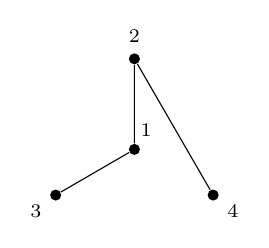
\begin{tikzpicture}[every node/.style={fill,circle,minimum size=4pt,inner sep=0}]
        \node[label={[shift={(0.15,0.05)},font=\scriptsize]1}] (1) at (0,0) {};
        \node[label={[shift={(0,0.1)},font=\scriptsize]2}] (2) at (0,1.15) {};
        \node[label={[shift={(-0.25,-0.4)},font=\scriptsize]3}] (3) at (-1,-0.58) {};
        \node[label={[shift={(0.25,-0.4)},font=\scriptsize]4}] (4) at (1,-0.58) {};
        \draw (1) -- (2) (1) -- (3) (2) -- (4);
      \end{tikzpicture}
    \end{minipage}
    \begin{minipage}{0.17\textwidth}
      \begin{tikzpicture}[every node/.style={fill,circle,minimum size=4pt,inner sep=0}]
        \node[label={[shift={(0.15,0.05)},font=\scriptsize]1}] (1) at (0,0) {};
        \node[label={[shift={(0,0.1)},font=\scriptsize]2}] (2) at (0,1.15) {};
        \node[label={[shift={(-0.25,-0.4)},font=\scriptsize]3}] (3) at (-1,-0.58) {};
        \node[label={[shift={(0.25,-0.4)},font=\scriptsize]4}] (4) at (1,-0.58) {};
        \draw (1) -- (2) (1) -- (3) (3) -- (4);
      \end{tikzpicture}
    \end{minipage}
    \begin{minipage}{0.17\textwidth}
      \begin{tikzpicture}[every node/.style={fill,circle,minimum size=4pt,inner sep=0}]
        \node[label={[shift={(0.15,0.05)},font=\scriptsize]1}] (1) at (0,0) {};
        \node[label={[shift={(0,0.1)},font=\scriptsize]2}] (2) at (0,1.15) {};
        \node[label={[shift={(-0.25,-0.4)},font=\scriptsize]3}] (3) at (-1,-0.58) {};
        \node[label={[shift={(0.25,-0.4)},font=\scriptsize]4}] (4) at (1,-0.58) {};
        \draw (1) -- (2) (1) -- (4) (3) -- (4);
      \end{tikzpicture}
    \end{minipage}
    \\
    \begin{minipage}{0.17\textwidth}
      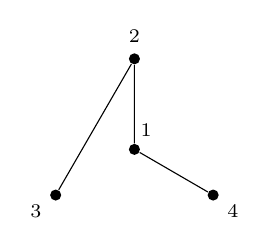
\begin{tikzpicture}[every node/.style={fill,circle,minimum size=4pt,inner sep=0}]
        \node[label={[shift={(0.15,0.05)},font=\scriptsize]1}] (1) at (0,0) {};
        \node[label={[shift={(0,0.1)},font=\scriptsize]2}] (2) at (0,1.15) {};
        \node[label={[shift={(-0.25,-0.4)},font=\scriptsize]3}] (3) at (-1,-0.58) {};
        \node[label={[shift={(0.25,-0.4)},font=\scriptsize]4}] (4) at (1,-0.58) {};
        \draw (1) -- (2) (1) -- (4) (2) -- (3);
      \end{tikzpicture}
    \end{minipage}
    \begin{minipage}{0.17\textwidth}
      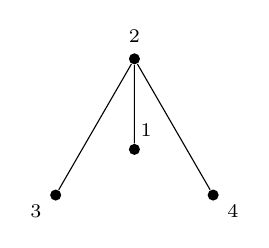
\begin{tikzpicture}[every node/.style={fill,circle,minimum size=4pt,inner sep=0}]
        \node[label={[shift={(0.15,0.05)},font=\scriptsize]1}] (1) at (0,0) {};
        \node[label={[shift={(0,0.1)},font=\scriptsize]2}] (2) at (0,1.15) {};
        \node[label={[shift={(-0.25,-0.4)},font=\scriptsize]3}] (3) at (-1,-0.58) {};
        \node[label={[shift={(0.25,-0.4)},font=\scriptsize]4}] (4) at (1,-0.58) {};
        \draw (1) -- (2) (2) -- (3) (2) -- (4);
      \end{tikzpicture}
    \end{minipage}
    \begin{minipage}{0.17\textwidth}
      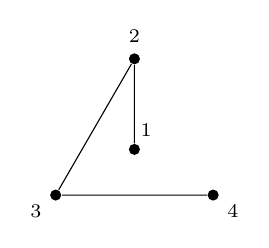
\begin{tikzpicture}[every node/.style={fill,circle,minimum size=4pt,inner sep=0}]
        \node[label={[shift={(0.15,0.05)},font=\scriptsize]1}] (1) at (0,0) {};
        \node[label={[shift={(0,0.1)},font=\scriptsize]2}] (2) at (0,1.15) {};
        \node[label={[shift={(-0.25,-0.4)},font=\scriptsize]3}] (3) at (-1,-0.58) {};
        \node[label={[shift={(0.25,-0.4)},font=\scriptsize]4}] (4) at (1,-0.58) {};
        \draw (1) -- (2) (2) -- (3) (3) -- (4);
      \end{tikzpicture}
    \end{minipage}
    \begin{minipage}{0.17\textwidth}
      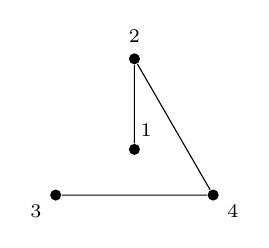
\begin{tikzpicture}[every node/.style={fill,circle,minimum size=4pt,inner sep=0}]
        \node[label={[shift={(0.15,0.05)},font=\scriptsize]1}] (1) at (0,0) {};
        \node[label={[shift={(0,0.1)},font=\scriptsize]2}] (2) at (0,1.15) {};
        \node[label={[shift={(-0.25,-0.4)},font=\scriptsize]3}] (3) at (-1,-0.58) {};
        \node[label={[shift={(0.25,-0.4)},font=\scriptsize]4}] (4) at (1,-0.58) {};
        \draw (1) -- (2) (2) -- (4) (3) -- (4);
      \end{tikzpicture}
    \end{minipage}
    \\
    \begin{minipage}{0.17\textwidth}
      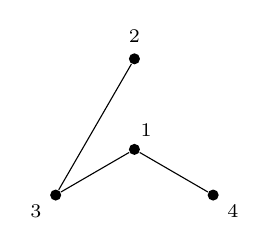
\begin{tikzpicture}[every node/.style={fill,circle,minimum size=4pt,inner sep=0}]
        \node[label={[shift={(0.15,0.05)},font=\scriptsize]1}] (1) at (0,0) {};
        \node[label={[shift={(0,0.1)},font=\scriptsize]2}] (2) at (0,1.15) {};
        \node[label={[shift={(-0.25,-0.4)},font=\scriptsize]3}] (3) at (-1,-0.58) {};
        \node[label={[shift={(0.25,-0.4)},font=\scriptsize]4}] (4) at (1,-0.58) {};
        \draw (1) -- (3) (1) -- (4) (2) -- (3);
      \end{tikzpicture}
    \end{minipage}
    \begin{minipage}{0.17\textwidth}
      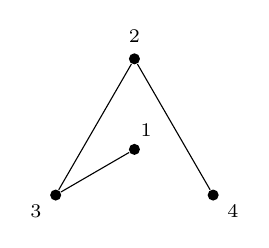
\begin{tikzpicture}[every node/.style={fill,circle,minimum size=4pt,inner sep=0}]
        \node[label={[shift={(0.15,0.05)},font=\scriptsize]1}] (1) at (0,0) {};
        \node[label={[shift={(0,0.1)},font=\scriptsize]2}] (2) at (0,1.15) {};
        \node[label={[shift={(-0.25,-0.4)},font=\scriptsize]3}] (3) at (-1,-0.58) {};
        \node[label={[shift={(0.25,-0.4)},font=\scriptsize]4}] (4) at (1,-0.58) {};
        \draw (1) -- (3) (2) -- (3) (2) -- (4);
      \end{tikzpicture}
    \end{minipage}
    \begin{minipage}{0.17\textwidth}
      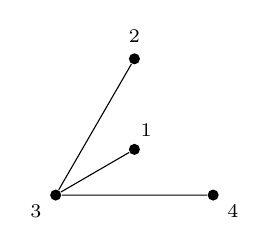
\begin{tikzpicture}[every node/.style={fill,circle,minimum size=4pt,inner sep=0}]
        \node[label={[shift={(0.15,0.05)},font=\scriptsize]1}] (1) at (0,0) {};
        \node[label={[shift={(0,0.1)},font=\scriptsize]2}] (2) at (0,1.15) {};
        \node[label={[shift={(-0.25,-0.4)},font=\scriptsize]3}] (3) at (-1,-0.58) {};
        \node[label={[shift={(0.25,-0.4)},font=\scriptsize]4}] (4) at (1,-0.58) {};
        \draw (1) -- (3) (2) -- (3) (3) -- (4);
      \end{tikzpicture}
    \end{minipage}
    \begin{minipage}{0.17\textwidth}
      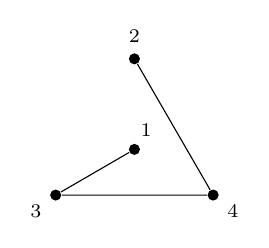
\begin{tikzpicture}[every node/.style={fill,circle,minimum size=4pt,inner sep=0}]
        \node[label={[shift={(0.15,0.05)},font=\scriptsize]1}] (1) at (0,0) {};
        \node[label={[shift={(0,0.1)},font=\scriptsize]2}] (2) at (0,1.15) {};
        \node[label={[shift={(-0.25,-0.4)},font=\scriptsize]3}] (3) at (-1,-0.58) {};
        \node[label={[shift={(0.25,-0.4)},font=\scriptsize]4}] (4) at (1,-0.58) {};
        \draw (1) -- (3) (2) -- (4) (3) -- (4);
      \end{tikzpicture}
    \end{minipage}
    \\
    \begin{minipage}{0.17\textwidth}
      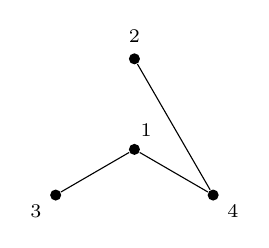
\begin{tikzpicture}[every node/.style={fill,circle,minimum size=4pt,inner sep=0}]
        \node[label={[shift={(0.15,0.05)},font=\scriptsize]1}] (1) at (0,0) {};
        \node[label={[shift={(0,0.1)},font=\scriptsize]2}] (2) at (0,1.15) {};
        \node[label={[shift={(-0.25,-0.4)},font=\scriptsize]3}] (3) at (-1,-0.58) {};
        \node[label={[shift={(0.25,-0.4)},font=\scriptsize]4}] (4) at (1,-0.58) {};
        \draw (1) -- (3) (1) -- (4) (2) -- (4);
      \end{tikzpicture}
    \end{minipage}
    \begin{minipage}{0.17\textwidth}
      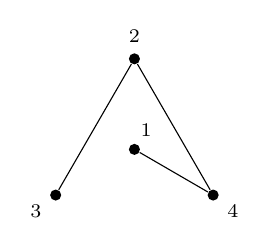
\begin{tikzpicture}[every node/.style={fill,circle,minimum size=4pt,inner sep=0}]
        \node[label={[shift={(0.15,0.05)},font=\scriptsize]1}] (1) at (0,0) {};
        \node[label={[shift={(0,0.1)},font=\scriptsize]2}] (2) at (0,1.15) {};
        \node[label={[shift={(-0.25,-0.4)},font=\scriptsize]3}] (3) at (-1,-0.58) {};
        \node[label={[shift={(0.25,-0.4)},font=\scriptsize]4}] (4) at (1,-0.58) {};
        \draw (1) -- (4) (2) -- (3) (2) -- (4);
      \end{tikzpicture}
    \end{minipage}
    \begin{minipage}{0.17\textwidth}
      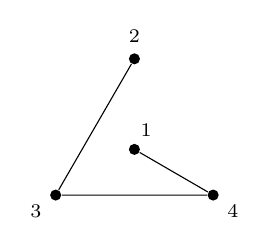
\begin{tikzpicture}[every node/.style={fill,circle,minimum size=4pt,inner sep=0}]
        \node[label={[shift={(0.15,0.05)},font=\scriptsize]1}] (1) at (0,0) {};
        \node[label={[shift={(0,0.1)},font=\scriptsize]2}] (2) at (0,1.15) {};
        \node[label={[shift={(-0.25,-0.4)},font=\scriptsize]3}] (3) at (-1,-0.58) {};
        \node[label={[shift={(0.25,-0.4)},font=\scriptsize]4}] (4) at (1,-0.58) {};
        \draw (1) -- (4) (2) -- (3) (3) -- (4);
      \end{tikzpicture}
    \end{minipage}
    \begin{minipage}{0.17\textwidth}
      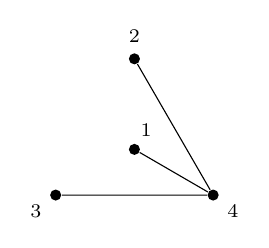
\begin{tikzpicture}[every node/.style={fill,circle,minimum size=4pt,inner sep=0}]
        \node[label={[shift={(0.15,0.05)},font=\scriptsize]1}] (1) at (0,0) {};
        \node[label={[shift={(0,0.1)},font=\scriptsize]2}] (2) at (0,1.15) {};
        \node[label={[shift={(-0.25,-0.4)},font=\scriptsize]3}] (3) at (-1,-0.58) {};
        \node[label={[shift={(0.25,-0.4)},font=\scriptsize]4}] (4) at (1,-0.58) {};
        \draw (1) -- (4) (2) -- (4) (3) -- (4);
      \end{tikzpicture}
    \end{minipage}
    \caption{The 16 spanning trees of $K_4$.}
  \end{figure}
\end{example}

\begin{algorithm}[Encoding]
  Let $S \subseteq \NN$ be finite with $|S| \geq 2$, and let $n = |S|$.
  Given a tree $T$ on $S$, we compute the \emph{Pr\"ufer sequence} $P = (p_1, p_2, \dots, p_{n-2})$ that corresponds to $T$ as follows.
  \begin{enumerate}[label=\arabic*.]
    \item For $i \gets 1, 2, \dots, n-2$, perform the following steps.
    \begin{enumerate}[label*=\arabic*.]
      \item Let $u$ be the smallest vertex of $T$ that is a leaf, and let $v$ be the unique neighbor of $u$.
      \item Let $p_i \gets v$.
      \item Remove $u$ from $T$.
    \end{enumerate}
    \item Return $P = (p_1, p_2, \dots, p_{n-2})$.
  \end{enumerate}
\end{algorithm}

\begin{algorithm}[Decoding]
  Let $S \subseteq \NN$ be finite with $|S| \geq 2$, and let $n = |S|$.
  Given a Pr\"ufer sequence $P = (p_1, p_2, \dots, p_{n-2})$ in $S$, we compute the tree $T$ on $S$ that corresponds to $P$.
  \begin{enumerate}[label=\arabic*.]
    \item Let $T$ be an empty graph on $S$, and let $Q \gets S$.
    \item For $i \gets 1, 2, \dots, n-2$, perform the following steps.
    \begin{enumerate}[label*=\arabic*.]
      \item Let $u$ be the smallest vertex in $Q \setminus \{p_i, p_{i+1}, \dots, p_{n-2}\}$.
      \item Let $v \gets p_i$.
      \item Add the edge $(u, v)$ to $T$.
      \item Remove $u$ from $Q$.
    \end{enumerate}
    \item Let $u$ and $v$ be the two vertices left in $Q$.
    Add the edge $(u, v)$ to $T$.
    \item Return $T$.
  \end{enumerate}
\end{algorithm}

\begin{theorem}[Cayley's Formula]
  $\tau(K_n) = n^{n-2}$.
\end{theorem}

\section{March 2, 2021}
\subsection{Minimum Spanning Tree}
\begin{algorithm}[Boru\r{v}ka]
  Given a weighted graph $G$ with $n$ vertices and $m$ edges, this algorithm computes a minimum spanning tree $T$ of $G$.
  \begin{enumerate}[label*=\arabic*.]
    \item Let $T$ be an empty graph on the vertices of $G$.
    \item Perform the following steps until $T$ is connected.
    \begin{enumerate}[label*=\arabic*.]
      \item Let $F$ be the forest that contains the smallest edge incident of each vertex of $G$.
      \item Add each edge in $F$ to $T$, and remove each edge in $F$ from $G$.
    \end{enumerate}
    \item Return $T$.
  \end{enumerate}
\end{algorithm}

\begin{algorithm}[Prim]
  Given a weighted graph $G$, this algorithm computes a minimum spanning tree $T$ of $G$.
  \begin{enumerate}[label*=\arabic*.]
    \item Let $T$ be an empty graph on the vertices of $G$.
    \item Choose an arbitrary vertex $s \in V$, and let $Q \gets V \setminus \{s\}$.
    \item For each vertex $v$, let $d[v] \gets w(s, v)$ if $v$ is adjacent to $s$; let $d[v] \gets \infty$ otherwise.
    \item For $i \gets 1, 2, \dots, n-1$, perform the following steps.
    \begin{enumerate}[label*=\arabic*.]
      \item Find a vertex $u \in Q$ such that $d[u]$ is minimized.
      \item For each neighbor $v$ of $u$, if $d[u] + w(u, v) < d[v]$, let $d[v] \gets d[u] + w(u, v)$.
      \item Remove $u$ from $Q$, and add $(u, v)$ to $T$.
    \end{enumerate}
    \item Return $T$.
  \end{enumerate}
\end{algorithm}

\begin{algorithm}[Kruskal]
  Given a weighted graph $G$ with $n$ vertices, this algorithm computes a minimum spanning tree $T$ of $G$.
  \begin{enumerate}[label*=\arabic*.]
    \item Let $T$ be an empty graph on the vertices of $G$.
    \item For $i \gets 1, 2, \dots, n-1$, perform the following steps.
    \begin{enumerate}[label*=\arabic*.]
      \item Choose a minimum-weight edge $(u, v)$ such that $u$ and $v$ lie on different components of $T$.
      \item Add $(u, v)$ to $T$.
    \end{enumerate}
    \item Return $T$.
  \end{enumerate}
\end{algorithm}

\subsection{Travelling Salesperson Problem with Triangle Inequality}
The \emph{travelling salesperson problem (TSP)} aims to find a Hamiltonian cycle with minimum weight in a complete weighted graph $G = (V, E, w)$.
In this section, we propose an algorithm that computes a $2$-approximate solution to TSP in which triangle inequality holds, i.e., we have $w(x, y) \leq w(x, z) + w(y, z)$ for all vertices $x, y, z$.

\begin{algorithm}[2-Approximation for TSP with Triangle Inequality]
  For any complete weighted graph $G = (V, E, w)$ in which triangle inequality holds, this algorithm computes a $2$-approximate solution to TSP.
  \begin{enumerate}[label=\arabic*.]
    \item Compute a minimum spanning tree $T$ of $G$, and choose an arbitrary vertex $s$.
    \item Let $P$ be an arbitrary preorder of $T$ rooted at $s$.
    \item Return $P$.
  \end{enumerate}
\end{algorithm}

\subsection{Shortest-Path Tree}
\begin{algorithm}[Dijkstra]
  Let $G = (V, E)$ be a directed graph with $n$ vertices and $m$ edges, let $w: E \to \RR_{\geq 0}$ be a nonnegative weight function, and let $s \in V$.
  This algorithm computes a shortest-path tree of $G$ rooted at $s$.
  \begin{enumerate}[label=\arabic*.]
    \item Initialization.
    \begin{enumerate}[label*=\arabic*.]
      \item For each vertex $v$, let $\pi[v] \gets v$.
      \item For each vertex $v$, let $d[v] \gets \infty$ if $v \neq s$, and let $d[s] \gets 0$.
      \item Let $Q \gets V$.
    \end{enumerate}
    \item Perform the following steps until $Q$ becomes empty.
    \begin{enumerate}[label*=\arabic*.]
      \item Find a vertex $u \in Q$ such that $d[u]$ is minimized.
      \item For each neighbor $v$ of $u$, if $d[u] + w(u, v) < d[v]$, let $\pi[v] \gets u$ and $d[v] \gets d[u] + w(u, v)$.
      \item Remove $u$ from $Q$.
    \end{enumerate}
    \item Return $(\pi, d)$.
  \end{enumerate}
\end{algorithm}

\begin{algorithm}[Bellman--Ford]
  Let $G = (V, E)$ be a directed graph with $n$ vertices and $m$ edges, let $w: E \to \RR$ be a weight function, and let $s \in V$.
  This algorithm detects whether there is a negative cycle in $G$ and computes a shortest-path tree of $G$ rooted at $s$.
  \begin{enumerate}[label=\arabic*.]
    \item Initialization.
    \begin{enumerate}[label*=\arabic*.]
      \item For each vertex $v$, let $\pi[v] \gets v$.
      \item For each vertex $v$, let $d[v] \gets \infty$ if $v \neq s$, and let $d[s] \gets 0$.
    \end{enumerate}
    \item For $i \gets 1, 2, \dots, n - 1$, perform the following step.
    \begin{enumerate}[label*=\arabic*.]
      \item For each edge $(u, v) \in E$, if $d[u] + w(u, v) < d[v]$, let $\pi[v] \gets u$ and $d[v] \gets d[u] + w(u, v)$.
    \end{enumerate}
    \item If there is an edge $(u, v) \in E$ such that $d[u] + w(u, v) < d[v]$, then report that a negative cycle exists.
    Otherwise, report that no negative cycles exist and return $(\pi, d)$.
  \end{enumerate}
\end{algorithm}

\subsection{Minimum Routing Cost Spanning Tree}
The \emph{routing cost} of a weighted tree $T = (V, E, w)$ is defined by
\begin{equation*}
  C(T) = \sum_{u \in V} \sum_{v \in V} w(u, v).
\end{equation*}
For a weighted graph $G$, a \emph{minimum routing cost spanning tree (MRCT)} of $G$ is a spanning tree of $G$ with minimum routing weight.
The \emph{routing load} of an edge $(u, v)$ with respect to a spanning tree $T$ is defined by
\begin{equation*}
  \ell_T(u, v) = 2|R||S|,
\end{equation*}
where $R$ and $S$ are the two components of the graph obtained from $T$ by removing $(u, v)$.
We have
\begin{equation*}
  C(T) = \sum_{(u, v) \in E} \ell_T(u, v) w(u, v).
\end{equation*}
Since the routing loads of all edges can be computed in linear time by depth first search in $T$, the routing cost of $T$ can be computed in linear time.

\section{March 9, 2021}
\subsection{Median}
A \emph{median} of a weighted graph $G = (V, E, w)$ is a vertex $r$ such that
\begin{equation*}
  r \in \argmin_{u \in V} \sum_{v \in V} w(u, v).
\end{equation*}
One can find that a shortest-path tree rooted at median is a 2-approximation of the MRCT of the graph.

\subsection{Centroid}
If the removal of a vertex $r$ from a tree $T$ causes each component contains at most half of the vertices, then the vertex $r$ is called a \emph{centroid} of $T$.

\end{document}
